%%%%%%%%%%%%%%%%%%%%%%%%%%%%% Thesis.tex %%%%%%%%%%%%%%%%%%%%%%%%%%%%%%%
%                                                                      %
%  ---------- Master of Science Dissertation template ----------       %
%                                                                      %
%  Template for the Master Thesis according to the regulations         %
%  published by the Scientific Council at IST.                         %
%                                                                      %
%  For up-to-date regulations, please refer to                         %
%  http://cd.ist.utl.pt/files/publico/academicos/guia_dissertacao.pdf  %
%                                                                      %
%       Andre C. Marta                                                 %
%       Area Cientifica de Mecanica Aplicada e Aeroespacial            %
%       Departamento de Engenharia Mecanica                            %
%       Instituto Superior Tecnico                                     %
%       Av. Rovisco Pais                                               %
%       1049-001 Lisboa                                                %
%       Portugal                                                       %
%       Tel: +351 21 841 9466                                          %
%                        3466 (extension)                              %
%       Email: andre.marta@ist.utl.pt                                  %
%                                                                      %
%  Created:       Jan 20, 2011                                         %
%  Last Modified: Jan 24, 2011                                         %
%                                                                      %
%%%%%%%%%%%%%%%%%%%%%%%%%%%%%%%%%%%%%%%%%%%%%%%%%%%%%%%%%%%%%%%%%%%%%%%%
%                                                                      %
% To generate the PDF file, type "make" at the terminal prompt.        %
%                                                                      %
% The IST template LaTeX package was created by the author             %
% and it can be downloaded from:                                       %
% https://fenix.ist.utl.pt/homepage/ist31052/                          %
%                                                                      %
% The external packages can be downloaded from                         %
% the Comprehensive TeX Archive Network at http://www.ctan.org/        %
%                                                                      %
% List of LaTex symbols:                                               %
% http://www.ctan.org/tex-archive/info/symbols/comprehensive/          %
%                                                                      %
% Help with LaTex can be found at                                      %
% http://www.giss.nasa.gov/tools/latex/ltx-2.html                      %
% http://en.wikibooks.org/wiki/LaTeX                                   %
%%%%%%%%%%%%%%%%%%%%%%%%%%%%%%%%%%%%%%%%%%%%%%%%%%%%%%%%%%%%%%%%%%%%%%%%

%%%%%%%%%%%%%%%%%%%%%%%%%%%%%%%%%%%%%%%%%%%%%%%%%%%%%%%%%%%%%%%%%%%%%%%%
%     Preamble                                                         %
%%%%%%%%%%%%%%%%%%%%%%%%%%%%%%%%%%%%%%%%%%%%%%%%%%%%%%%%%%%%%%%%%%%%%%%%

% ----------------------------------------------------------------------
%  Set the document class
% ----------------------------------------------------------------------
\documentclass[10pt,a4paper,twoside]{report}

% ----------------------------------------------------------------------
% Define external packages, language, margins, fonts and new commands
% ----------------------------------------------------------------------
%%%%%%%%%%%%%%%%%%%%%%%%%%%%%%%%%%%%%%%%%%%%%%%%%%%%%%%%%%%%%%%%%%%%%%%%
%                                                                      %
%     File: Thesis_Preamble.tex                                        %
%     Tex Master: Thesis.tex                                           %
%                                                                      %
%     Author: Andre C. Marta                                           %
%     Last modified : 24 Jan 2011                                      %
%                                                                      %
%%%%%%%%%%%%%%%%%%%%%%%%%%%%%%%%%%%%%%%%%%%%%%%%%%%%%%%%%%%%%%%%%%%%%%%%

% ----------------------------------------------------------------------
% Define document language.
% ----------------------------------------------------------------------

% 'inputenc' package
%
% Accept different input encodings.
% http://www.ctan.org/tex-archive/macros/latex/base/
%
% > allows typing non-english text in LaTeX sources.
%
% ******************************* SELECT *******************************
%\usepackage[latin1]{inputenc} % <<<<< Windows
\usepackage[utf8]{inputenc}   % <<<<< Linux
% ******************************* SELECT *******************************


% 'babel' package
%
% Multilingual support for Plain TeX or LaTeX.
% http://www.ctan.org/tex-archive/macros/latex/required/babel/
%
% > sets the variable names according to the language selected
%
% ******************************* SELECT *******************************
%\usepackage[portuguese]{babel} % <<<<< Portuguese
\usepackage[english]{babel} % <<<<< English
% ******************************* SELECT *******************************


% List of LaTeX variable names: \abstractname, \appendixname, \bibname,
%   \chaptername, \contentsname, \listfigurename, \listtablename, ...)
% http://www.tex.ac.uk/cgi-bin/texfaq2html?label=fixnam
%
% Changing the words babel uses (uncomment and redefine as necessary...)
%
\newcommand{\acknowledgments}{@undefined} % new LaTeX variable name
%
% > English
%
\addto\captionsenglish{\renewcommand{\acknowledgments}{Acknowledgments}}
%\addto\captionsenglish{\renewcommand{\listtablename}{List of Tables}}
%\addto\captionsenglish{\renewcommand{\listfigurename}{List of Figures}}
%\addto\captionsenglish{\renewcommand{\nomname}{Nomenclature}}
%\addto\captionsenglish{\renewcommand{\appendixname}{Appendix}}
%\addto\captionsenglish{\renewcommand{\bibname}{References}} % Bibliography

% > Portuguese
%
\addto\captionsportuguese{\renewcommand{\acknowledgments}{Agradecimentos}}
%\addto\captionsportuguese{\renewcommand{\listtablename}{Lista de Figuras}}
%\addto\captionsportuguese{\renewcommand{\listfigurename}{Lista de Tabelas}}
\addto\captionsportuguese{\renewcommand{\nomname}{Lista de S\'{i}mbolos}} % Nomenclatura
%\addto\captionsportuguese{\renewcommand{\appendixname}{Anexo}} % Apendice
%\addto\captionsportuguese{\renewcommand{\bibname}{Refer\^{e}ncias}} % Bibliografia


% ----------------------------------------------------------------------
% Define default and cover page fonts.
% ----------------------------------------------------------------------

% Use Arial font as default
%
\renewcommand{\rmdefault}{phv}
\renewcommand{\sfdefault}{phv}

% Define cover page fonts
%
%         encoding     family       series      shape
%  \usefont{T1}     {phv}=helvetica  {b}=bold    {n}=normal
%                   {ptm}=times      {m}=normal  {sl}=slanted
%                                                {it}=italic
% see more examples at
% http://julien.coron.free.fr/languages/latex/fonts/
%
\def\FontLn{% 16 pt normal
  \usefont{T1}{phv}{m}{n}\fontsize{16pt}{16pt}\selectfont}
\def\FontLb{% 16 pt bold
  \usefont{T1}{phv}{b}{n}\fontsize{16pt}{16pt}\selectfont}
\def\FontMn{% 14 pt normal
  \usefont{T1}{phv}{m}{n}\fontsize{14pt}{14pt}\selectfont}
\def\FontMb{% 14 pt bold
  \usefont{T1}{phv}{b}{n}\fontsize{14pt}{14pt}\selectfont}
\def\FontSn{% 12 pt normal
  \usefont{T1}{phv}{m}{n}\fontsize{12pt}{12pt}\selectfont}


% ----------------------------------------------------------------------
% Define page margins and line spacing.
% ----------------------------------------------------------------------

% 'geometry' package
%
% Flexible and complete interface to document dimensions.
% http://www.ctan.org/tex-archive/macros/latex/contrib/geometry/
%
% > set the page margins (2.5cm minimum in every side, as per IST rules)
%
\usepackage{geometry}	
\geometry{verbose,tmargin=2.5cm,bmargin=2.5cm,lmargin=2.5cm,rmargin=2.5cm}

% 'setspace' package
%
% Set space between lines.
% http://www.ctan.org/tex-archive/macros/latex/contrib/setspace/
%
% > allow setting line spacing (line spacing of 1.5, as per IST rules)
%
\usepackage{setspace}
\renewcommand{\baselinestretch}{1.5}


% ----------------------------------------------------------------------
% Include external packages.
% Note that not all of these packages may be available on all system
% installations. If necessary, include the .sty files locally in
% the <jobname>.tex file directory.
% ----------------------------------------------------------------------

% 'graphicx' package
%
% Enhanced support for graphics.
% http://www.ctan.org/tex-archive/macros/latex/required/graphics/
%
% > extends arguments of the \includegraphics command
%
\usepackage{graphicx}


% 'color' package
%
% Colour control for LaTeX documents.
% http://www.ctan.org/tex-archive/macros/latex/required/graphics/
%
% > defines color macros: \color{<color name>}
%
%\usepackage{color}


% 'amsmath' package
%
% Mathematical enhancements for LaTeX.
% http://www.ctan.org/tex-archive/macros/latex/required/amslatex/
%
% > American Mathematical Society plain Tex macros
%
\usepackage{amsmath}  % AMS mathematical facilities for LaTeX.
\usepackage{amsthm}   % Typesetting theorems (AMS style).
\usepackage{amsfonts} % 


% 'wrapfig' package
%
% Produces figures which text can flow around.
% http://www.ctan.org/tex-archive/macros/latex/contrib/wrapfig/
%
% > wrap figures/tables in text (i.e., Di Vinci style)
%
% \usepackage{wrapfig}


% 'subfigure' package
%
% Deprecated: Figures divided into subfigures.
% http://www.ctan.org/tex-archive/obsolete/macros/latex/contrib/subfigure/
%
% > subcaptions for subfigures
%
\usepackage{subfigure}


% 'subfigmat' package
%
% Automates layout when using the subfigure package.
% http://www.ctan.org/tex-archive/macros/latex/contrib/subfigmat/
%
% > matrices of similar subfigures
%
\usepackage{subfigmat}


% 'url' package
%
% Verbatim with URL-sensitive line breaks.
% http://www.ctan.org/tex-archive/macros/latex/contrib/url/
%
% > URLs in BibTex
%
% \usepackage{url}


% 'varioref' package
%
% Intelligent page references.
% http://www.ctan.org/tex-archive/macros/latex/required/tools/
%
% > smart page, figure, table and equation referencing
%
%\usepackage{varioref}


% 'dcolumn' package
%
% Align on the decimal point of numbers in tabular columns.
% http://www.ctan.org/tex-archive/macros/latex/required/tools/
%
% > decimal-aligned tabular math columns
%
\usepackage{dcolumn}
\newcolumntype{d}{D{.}{.}{-1}} % column aligned by the point separator '.'
\newcolumntype{e}{D{E}{E}{-1}} % column aligned by the exponent 'E'


% '' package
%
% Reimplementation of and extensions to LaTeX verbatim.
% http://www.ctan.org/tex-archive/macros/latex/required/tools/
%
% > provides the verbatim environment (\begin{verbatim},\end{verbatim})
%   and a comment environment (\begin{comment},  \end{comment})
%
% \usepackage{verbatim}


% 'moreverb' package
%
% Extended verbatim.
% http://www.ctan.org/tex-archive/macros/latex/contrib/moreverb/
%
% > supports tab expansion and line numbering
%
% \usepackage{moreverb}



% 'nomencl' package
%
% Produce lists of symbols as in nomenclature.
% http://www.ctan.org/tex-archive/macros/latex/contrib/nomencl/
%
% The nomencl package makes use of the MakeIndex program
% in order to produce the nomenclature list.
%
% Nomenclature
% 1) On running the file through LATEX, the command \makenomenclature
%    in the preamble instructs it to create/open the nomenclature file
%    <jobname>.nlo corresponding to the LATEX file <jobname>.tex and
%    writes the information from the \nomenclature commands to this file.
% 2) The next step is to invoke MakeIndex in order to produce the
%    <jobname>.nls file. This can be achieved by making use of the
%    command: makeindex <jobname>.nlo -s nomencl.ist -o <jobname>.nls
% 3) The last step is to invoke LATEX on the <jobname>.tex file once
%    more. There, the \printnomenclature in the document will input the
%    <jobname>.nls file and process it according to the given options.
%
% http://www-h.eng.cam.ac.uk/help/tpl/textprocessing/nomencl.pdf
%
\usepackage{nomencl}
\makenomenclature
%
% Group variables according to their symbol type
%
\RequirePackage{ifthen} 
\ifthenelse{\equal{\languagename}{english}}%
    { % English
    \renewcommand{\nomgroup}[1]{%
      \ifthenelse{\equal{#1}{R}}{%
        \item[\textbf{Roman symbols}]}{%
        \ifthenelse{\equal{#1}{G}}{%
          \item[\textbf{Greek symbols}]}{%
          \ifthenelse{\equal{#1}{S}}{%
            \item[\textbf{Subscripts}]}{%
            \ifthenelse{\equal{#1}{T}}{%
              \item[\textbf{Superscripts}]}{}}}}}%
    }{% Portuguese
    \renewcommand{\nomgroup}[1]{%
      \ifthenelse{\equal{#1}{R}}{%
        \item[\textbf{Simbolos romanos}]}{%
        \ifthenelse{\equal{#1}{G}}{%
          \item[\textbf{Simbolos gregos}]}{%
          \ifthenelse{\equal{#1}{S}}{%
            \item[\textbf{Subscritos}]}{%
            \ifthenelse{\equal{#1}{T}}{%
              \item[\textbf{Sobrescritos}]}{}}}}}%
    }%


% 'rotating' package
%
% Rotation tools, including rotated full-page floats.
% http://www.ctan.org/tex-archive/macros/latex/contrib/rotating/
%
% > show wide figures and tables in landscape format:
%   use \begin{sidewaystable} and \begin{sidewaysfigure}
%   instead of 'table' and 'figure', respectively.
%
\usepackage{rotating}


% 'hyperref' package
%
% Extensive support for hypertext in LaTeX.
% http://www.ctan.org/tex-archive/macros/latex/contrib/hyperref/
%
% > Extends the functionality of all the LATEX cross-referencing
%   commands (including the table of contents, bibliographies etc) to
%   produce \special commands which a driver can turn into hypertext
%   links; Also provides new commands to allow the user to write adhoc
%   hypertext links, including those to external documents and URLs.
%
\usepackage[pdftex]{hyperref} % enhance documents that are to be
                              % output as HTML and PDF
\hypersetup{colorlinks,       % color text of links and anchors,
                              % eliminates borders around links
%            linkcolor=red,    % color for normal internal links
            linkcolor=black,  % color for normal internal links
            anchorcolor=black,% color for anchor text
%            citecolor=green,  % color for bibliographical citations
            citecolor=black,  % color for bibliographical citations
%            filecolor=magenta,% color for URLs which open local files
            filecolor=black,  % color for URLs which open local files
%            menucolor=red,    % color for Acrobat menu items
            menucolor=black,  % color for Acrobat menu items
%            pagecolor=red,    % color for links to other pages
            pagecolor=black,  % color for links to other pages
%            urlcolor=cyan,    % color for linked URLs
            urlcolor=black,   % color for linked URLs
	          bookmarks=true,         % create PDF bookmarks
	          bookmarksopen=false,    % don't expand bookmarks
	          bookmarksnumbered=true, % number bookmarks
	          pdftitle={Thesis},
            pdfauthor={Andre C. Marta},
            pdfsubject={Thesis Title},
            pdfkeywords={Thesis Keywords},
            pdfstartview=FitV,
            pdfdisplaydoctitle=true}


% 'hypcap' package
%
% Adjusting the anchors of captions.
% http://www.ctan.org/tex-archive/macros/latex/contrib/oberdiek/
%
% > fixes the problem with hyperref, that links to floats points
%   below the caption and not at the beginning of the float.
%
\usepackage[figure,table]{hypcap}


% 'natbib' package
%
% Flexible bibliography support.
% http://www.ctan.org/tex-archive/macros/latex/contrib/natbib/
%
% > produce author-year style citations
%
% \citet  and \citep  for textual and parenthetical citations, respectively
% \citet* and \citep* that print the full author list, and not just the abbreviated one
% \citealt is the same as \citet but without parentheses. Similarly, \citealp is \citep without parentheses
% \citeauthor
% \citeyear
% \citeyearpar
%
\usepackage{natbib}


% ----------------------------------------------------------------------
% Define new commands to assure consistent treatment throughout document
% ----------------------------------------------------------------------

\newcommand{\ud}{\mathrm{d}}                % total derivative
\newcommand{\degree}{\ensuremath{^\circ\,}} % degrees

% Abbreviations

\newcommand{\mcol}{\multicolumn}            % table format

\newcommand{\eqnref}[1]{(\ref{#1})}
\newcommand{\class}[1]{\texttt{#1}}
\newcommand{\package}[1]{\texttt{#1}}
\newcommand{\file}[1]{\texttt{#1}}
\newcommand{\BibTeX}{\textsc{Bib}\TeX}

% Typefaces ( example: {\bf Bold text here} )
%
% > pre-defined
%   \bf % bold face
%   \it % italic
%   \tt % typewriter
%
% > newly defined
\newcommand{\tr}[1]{{\ensuremath{\textrm{#1}}}}   % text roman
\newcommand{\tb}[1]{{\ensuremath{\textbf{#1}}}}   % text bold face
\newcommand{\ti}[1]{{\ensuremath{\textit{#1}}}}   % text italic
\newcommand{\mc}[1]{{\ensuremath{\mathcal{#1}}}}  % math calygraphy
\newcommand{\mco}[1]{{\ensuremath{\mathcalold{#1}}}}% math old calygraphy
\newcommand{\mr}[1]{{\ensuremath{\mathrm{#1}}}}   % math roman
\newcommand{\mb}[1]{{\ensuremath{\mathbf{#1}}}}   % math bold face
\newcommand{\bs}[1]{\ensuremath{\boldsymbol{#1}}} % math symbol
\def\bm#1{\mathchoice                             % math bold
  {\mbox{\boldmath$\displaystyle#1$}}%
  {\mbox{\boldmath$#1$}}%
  {\mbox{\boldmath$\scriptstyle#1$}}%
  {\mbox{\boldmath$\scriptscriptstyle#1$}}}
\newcommand{\boldcal}[1]{{\ensuremath{\boldsymbol{\mathcal{#1}}}}}% math bold calygraphy

 % file "Thesis_Preamble.tex"

%%%%%%%%%%%%%%%%%%%%%%%%%%%%%%%%%%%%%%%%%%%%%%%%%%%%%%%%%%%%%%%%%%%%%%%%
%     Begin Document                                                   %
%%%%%%%%%%%%%%%%%%%%%%%%%%%%%%%%%%%%%%%%%%%%%%%%%%%%%%%%%%%%%%%%%%%%%%%%
\begin{document}

% Set plain page style (no headers, footer with centered page number)
\pagestyle{plain}

% Set roman numbering (i,ii,...) before the start of chapters
\pagenumbering{roman}

% ----------------------------------------------------------------------
%  Cover page
% ----------------------------------------------------------------------
%%%%%%%%%%%%%%%%%%%%%%%%%%%%%%%%%%%%%%%%%%%%%%%%%%%%%%%%%%%%%%%%%%%%%%%%
%                                                                      %
%     File: Thesis_FrontCover.tex                                      %
%     Tex Master: Thesis.tex                                           %
%                                                                      %
%     Author: Andre C. Marta                                           %
%     Last modified : 21 Jan 2011                                      %
%                                                                      %
%%%%%%%%%%%%%%%%%%%%%%%%%%%%%%%%%%%%%%%%%%%%%%%%%%%%%%%%%%%%%%%%%%%%%%%%

\thispagestyle {empty}

% IST Logo
% parameters: bb=llx lly urx ury (bounding box), width=h_length, height=v_length, angle=angle, scale=factor, clip=true/false, draft=true/false. 

\includegraphics[bb=1.86cm 0cm 10cm 3.16cm,scale=0.56]{Logo}

\begin{center}
%
% Figure (Image or plot)
\vspace{1cm}
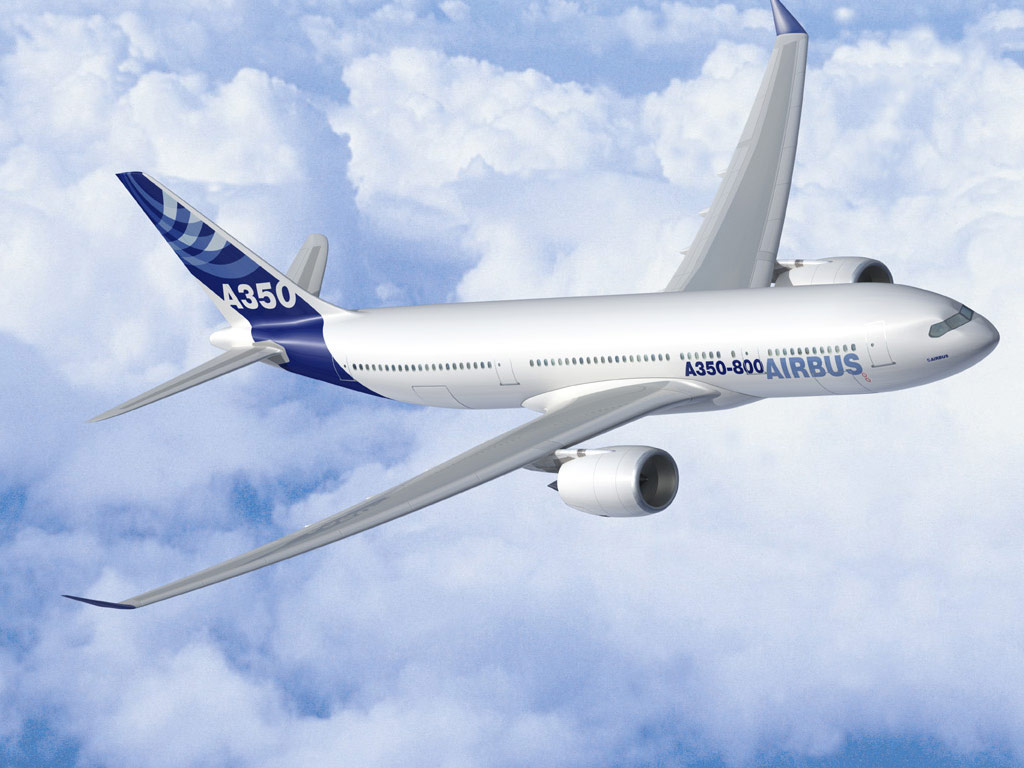
\includegraphics[height=50mm]{Figures/Airbus_A350.jpg}

% Title, author and degree
\vspace{0.8cm}
{\FontLb Título da Dissertação} \\
\vspace{0.2cm}
{\FontMn Subtítulo (facultativo)} \\
\vspace{1.9cm}
{\FontMb Nome Completo do Candidato} \\
\vspace{1.9cm}
{\FontLn Disserta\c{c}\~{a}o para a obten\c{c}\~{a}o de Grau de Mestre em} \\
\vspace{0.3cm}
{\FontLb Engenharia Aeroespacial} \\
\vspace{1.9cm}
{\FontMb J\'{u}ri} \\
\vspace{0.3cm}
{\FontSn %
\begin{tabular}{ll}
Presidente: & Nome do Presidente \\
Orientador: & Nome do Orientador \\
Co-orientador: & Nome do Co-orientador \\
Vogais: & Nome do Vogal 1 \\
        & Nome do Vogal 2 \\
        & Nome do Vogal 3 \\
\end{tabular} } \\
\vspace{1.1cm}
{\FontMb M\^{e}s e Ano} \\
%
\end{center}

\cleardoublepage

 % file "Thesis_FrontCover.tex"

% ----------------------------------------------------------------------
% Dedication page (optional)
% ----------------------------------------------------------------------
%%%%%%%%%%%%%%%%%%%%%%%%%%%%%%%%%%%%%%%%%%%%%%%%%%%%%%%%%%%%%%%%%%%%%%%%
%                                                                      %
%     File: Thesis_Dedication.tex                                      %
%     Tex Master: Thesis.tex                                           %
%                                                                      %
%     Author: Andre C. Marta                                           %
%     Last modified : 21 Jan 2011                                      %
%                                                                      %
%%%%%%%%%%%%%%%%%%%%%%%%%%%%%%%%%%%%%%%%%%%%%%%%%%%%%%%%%%%%%%%%%%%%%%%%

\null\vskip5cm%
\begin{flushright}
     Dedicated to someone special...
\end{flushright}
\vfill\newpage

\cleardoublepage

 % file "Thesis_Dedication.tex"

% ----------------------------------------------------------------------
%  Acknowledgments (optional)
% ----------------------------------------------------------------------
%%%%%%%%%%%%%%%%%%%%%%%%%%%%%%%%%%%%%%%%%%%%%%%%%%%%%%%%%%%%%%%%%%%%%%%%
%                                                                      %
%     File: Thesis_Acknowledgments.tex                                 %
%     Tex Master: Thesis.tex                                           %
%                                                                      %
%     Author: Andre C. Marta                                           %
%     Last modified : 21 Jan 2011                                      %
%                                                                      %
%%%%%%%%%%%%%%%%%%%%%%%%%%%%%%%%%%%%%%%%%%%%%%%%%%%%%%%%%%%%%%%%%%%%%%%%

\section*{\acknowledgments}

% Add entry in the table of contents as section
\addcontentsline{toc}{section}{\acknowledgments}

A few words about the university, financial support, research advisor, dissertation readers, faculty or other professors, lab mates, other friends and family...

\cleardoublepage

 % file "Thesis_Acknowledgements.tex"

% ----------------------------------------------------------------------
%  Abstract (both in English and Portuguese)
% ----------------------------------------------------------------------
%%%%%%%%%%%%%%%%%%%%%%%%%%%%%%%%%%%%%%%%%%%%%%%%%%%%%%%%%%%%%%%%%%%%%%%%
%                                                                      %
%     File: Thesis_Resumo.tex                                          %
%     Tex Master: Thesis.tex                                           %
%                                                                      %
%     Author: Andre C. Marta                                           %
%     Last modified : 21 Jan 2011                                      %
%                                                                      %
%%%%%%%%%%%%%%%%%%%%%%%%%%%%%%%%%%%%%%%%%%%%%%%%%%%%%%%%%%%%%%%%%%%%%%%%

\section*{Resumo}

% Add entry in the table of contents as section
\addcontentsline{toc}{section}{Resumo}

Inserir o resumo em Portugu\^{e}s aqui com o máximo de 250 palavras e acompanhado de 4 a 6 palavras-chave...

\vfill

\textbf{\Large Palavras-chave:} palavra-chave1, palavra-chave2,...

\cleardoublepage

 % file "Thesis_Resumo.tex"
%%%%%%%%%%%%%%%%%%%%%%%%%%%%%%%%%%%%%%%%%%%%%%%%%%%%%%%%%%%%%%%%%%%%%%%%
%                                                                      %
%     File: Thesis_Abstract.tex                                        %
%     Tex Master: Thesis.tex                                           %
%                                                                      %
%     Author: Andre C. Marta                                           %
%     Last modified : 21 Jan 2011                                      %
%                                                                      %
%%%%%%%%%%%%%%%%%%%%%%%%%%%%%%%%%%%%%%%%%%%%%%%%%%%%%%%%%%%%%%%%%%%%%%%%

\section*{Abstract}

% Add entry in the table of contents as section
\addcontentsline{toc}{section}{Abstract}

Insert your abstract here with a maximum of 250 words, followed by 4 to 6 keywords...

\vfill

\textbf{\Large Keywords:} keyword1, keyword2,...

\cleardoublepage

 % file "Thesis_Abstract.tex"

% ----------------------------------------------------------------------
%  Table of contents, list of tables, list of figures and nomenclature
% ----------------------------------------------------------------------

% Table of contents
%
\tableofcontents
\cleardoublepage 

% List of tables
%
% Generate list
\listoftables
% Add entry in the table of contents as section
\addcontentsline{toc}{section}{\listtablename}
\cleardoublepage 

% List of figures
%
% Generate list
\listoffigures
% Add entry in the table of contents as section
\addcontentsline{toc}{section}{\listfigurename}
\cleardoublepage 

% Nomenclature
%
% entries of nomenclature list
%%%%%%%%%%%%%%%%%%%%%%%%%%%%%%%%%%%%%%%%%%%%%%%%%%%%%%%%%%%%%%%%%%%%%%%%
%                                                                      %
%     File: Thesis_Nomenclature.tex                                    %
%     Tex Master: Thesis.tex                                           %
%                                                                      %
%     Author: Andre C. Marta                                           %
%     Last modified : 21 Jan 2011                                      %
%                                                                      %
%%%%%%%%%%%%%%%%%%%%%%%%%%%%%%%%%%%%%%%%%%%%%%%%%%%%%%%%%%%%%%%%%%%%%%%%
%
% The definitions can be placed anywhere in the document body
% and their order is sorted by <symbol> automatically when
% calling makeindex in the makefile
%
% The \glossary command has the following syntax:
%
% \glossary{entry}
%
% The \nomenclature command has the following syntax:
%
% \nomenclature[<prefix>]{<symbol>}{<description>}
%
% where <prefix> is used for fine tuning the sort order,
% <symbol> is the symbol to be described, and <description> is
% the actual description.

% ----------------------------------------------------------------------
% Roman symbols [r]
\nomenclature[ru]{$\bf u$}{Velocity vector.}
\nomenclature[ru]{$u,v,w$}{Velocity Cartesian components.}
\nomenclature[rp]{$p$}{Pressure.}
\nomenclature[rC]{$C_D$}{Coefficient of drag.}
\nomenclature[rC]{$C_L$}{Coefficient of lift.}
\nomenclature[rC]{$C_M$}{Coefficient of moment.}

% ----------------------------------------------------------------------
% Greek symbols [g]
\nomenclature[g]{$\rho$}{Density.}
\nomenclature[g]{$\alpha$}{Angle of attack.}
\nomenclature[g]{$\beta$}{Angle of side-slip.}
\nomenclature[g]{$\mu$}{Molecular viscosity coefficient.}
\nomenclature[g]{$\kappa$}{Thermal conductivity coefficient.}

% ----------------------------------------------------------------------
% Subscripts [s]
\nomenclature[s]{$x,y,z$}{Cartesian components.}
\nomenclature[s]{$i,j,k$}{Computational indexes.}
\nomenclature[s]{$\infty$}{Free-stream condition.}
\nomenclature[s]{ref}{Reference condition.}
\nomenclature[s]{$n$}{Normal component.}

% ----------------------------------------------------------------------
% Supercripts [t]
\nomenclature[t]{T}{Transpose.}
\nomenclature[t]{*}{Adjoint.}

 % file "Thesis_Nomenclature.tex"
%
% Insert glossary/nomenclature section produced by MakeIndex
\printnomenclature
% Add entry in the table of contents as section
\addcontentsline{toc}{section}{\nomname}
\cleardoublepage

% Set arabic numbering (1,2,...) after preface
%
\setcounter{page}{1}
\pagenumbering{arabic}

% ----------------------------------------------------------------------
%  Chapters
% ----------------------------------------------------------------------

%%%%%%%%%%%%%%%%%%%%%%%%%%%%%%%%%%%%%%%%%%%%%%%%%%%%%%%%%%%%%%%%%%%%%%%%
%                                                                      %
%     File: Thesis_Introduction.tex                                    %
%     Tex Master: Thesis.tex                                           %
%                                                                      %
%     Author: Andre C. Marta                                           %
%     Last modified : 21 Jan 2011                                      %
%                                                                      %
%%%%%%%%%%%%%%%%%%%%%%%%%%%%%%%%%%%%%%%%%%%%%%%%%%%%%%%%%%%%%%%%%%%%%%%%

\chapter{Introduction}
\label{chapter:introduction}

Insert your chapter material here...

% ----------------------------------------------------------------------
\section{Motivation}
\label{section:motivation}

Relevance of the subject...


% ----------------------------------------------------------------------
\section{State-of-the-art}
\label{section:state}

Insert your section material with the appropriate citations.
These can be cited in the following way: \\

Citation mode \#1 - \quad \cite{jameson:adjointns}

Citation mode \#2 - \quad \citet{jameson:adjointns}

Citation mode \#3 - \quad \citep{jameson:adjointns}


Citation mode \#4 - \quad \citet*{jameson:adjointns}

Citation mode \#5 - \quad \citep*{jameson:adjointns}


Citation mode \#6 - \quad \citealt{jameson:adjointns}

Citation mode \#7 - \quad \citealp{jameson:adjointns}


Citation mode \#8 - \quad \citeauthor{jameson:adjointns}

Citation mode \#9 - \quad \citeyear{jameson:adjointns}

Citation mode \#10 - \quad \citeyearpar{jameson:adjointns}


\subsection{Tables}
\label{subsection:tables}

Insert your subsection material and for instance a few tables...

\begin{table}[h!]
  \begin{center}
    \begin{tabular}{|c|c|}
      \hline
      item 1 & item 2 \\
      \hline
      item 3 & item 4 \\
      \hline
    \end{tabular}
  \end{center}
  \caption[Table caption shown in TOC]{Table caption}
  \label{table:simple}
\end{table}

Make reference to Table \ref{table:simple}.

\begin{table}[!htb]
  \begin{center}
    \begin{tabular}{lccc}
      Model           & $C_L$ & $C_D$ & $C_{M y}$ \\
      \hline
      Euler           & 0.083 & 0.021 & -0.110    \\
      Navier--Stokes  & 0.078 & 0.023 & -0.101    \\
      \hline
    \end{tabular}
  \end{center}
  \caption{Aerodynamic coefficients.}
  \label{tab:aeroCoeff}
\end{table}

Here is an example of a table with merging columns:

\begin{table}[!htb]
  \begin{center}
    \begin{tabular}[]{lrr}
      \hline
                     & \multicolumn{2}{c}{\underline{Virtual memory [MB]}} \\
                     & Euler       & Navier--Stokes \\
      \hline
      Wing only      &  1,000      &    2,000       \\
      Aircraft       &  5,000      &   10,000       \\
      (ratio)        & $5.0\times$ & $5.0\times$    \\
      \hline
    \end{tabular}
  \end{center}
  \caption{Memory usage comparison (in MB).}
  \label{tab:memory}
\end{table}


\subsection{Drawings}
\label{subsection:drawings}

Insert your subsection material and for instance a few drawings...

The schematic illustrated in Fig.~\ref{fig:algorithm} can represent some sort of algorithm.

\begin{figure}[!htb]
  \centering
  \scriptsize
%  \footnotesize 
%  \small
  \setlength{\unitlength}{0.9cm}
  \begin{picture}(8.5,6)
    \linethickness{0.3mm}

    \put(3,6){\vector(0,-1){1}}
    \put(3.5,5.4){$\bf \alpha$}
    \put(3,4.5){\oval(6,1){}}
    %\put(0,4){\framebox(6,1){}}
    \put(0.3,4.4){Grid Generation: \quad ${\bf x} = {\bf x}\left({\bf \alpha}\right)$}

    \put(3,4){\vector(0,-1){1}}
    \put(3.5,3.4){$\bf x$}
    \put(3,2.5){\oval(6,1){}}
    %\put(0,2){\framebox(6,1){}}
    \put(0.3,2.4){Flow Solver: \quad ${\cal R}\left({\bf x},{\bf q}\left({\bf x}\right)\right) = 0$}

    \put(6.0,2.5){\vector(1,0){1}}
    \put(6.4,3){$Y_1$}

    \put(3,2){\vector(0,-1){1}}
    \put(3.5,1.4){$\bf q$}
    \put(3,0.5){\oval(6,1){}}
    %\put(0,0){\framebox(6,1){}}
    \put(0.3,0.4){Structural Solver: \quad ${\cal M}\left({\bf x},{\bf q}\left({\bf x}\right)\right) = 0$}

    \put(6.0,0.5){\vector(1,0){1}}
    \put(6.4,1){$Y_2$}

    %\put(7.8,2.5){\oval(1.6,5){}}
    \put(7.0,0){\framebox(1.6,5){}}
    \put(7.1,2.5){Optimizer}
    \put(7.8,5){\line(0,1){1}}
    \put(7.8,6){\line(-1,0){4.8}}
  \end{picture}
  \caption{Schematic of some algorithm.}
  \label{fig:algorithm}
\end{figure}

\cleardoublepage

 % file "Thesis_Introduction.tex"

%\input{new_file} % add new .tex files for new chapters

%%%%%%%%%%%%%%%%%%%%%%%%%%%%%%%%%%%%%%%%%%%%%%%%%%%%%%%%%%%%%%%%%%%%%%%%
%                                                                      %
%     File: Thesis_Results.tex                                         %
%     Tex Master: Thesis.tex                                           %
%                                                                      %
%     Author: Andre C. Marta                                           %
%     Last modified : 21 Jan 2011                                      %
%                                                                      %
%%%%%%%%%%%%%%%%%%%%%%%%%%%%%%%%%%%%%%%%%%%%%%%%%%%%%%%%%%%%%%%%%%%%%%%%

\chapter{Results}
\label{chapter:results}

Insert your chapter material here, much like in \ref{chapter:introduction}

% ----------------------------------------------------------------------
\section{Figures}
\label{section:figures}

Insert your section material and possibly a few figures...

\begin{figure}[!htb]
  \centering
  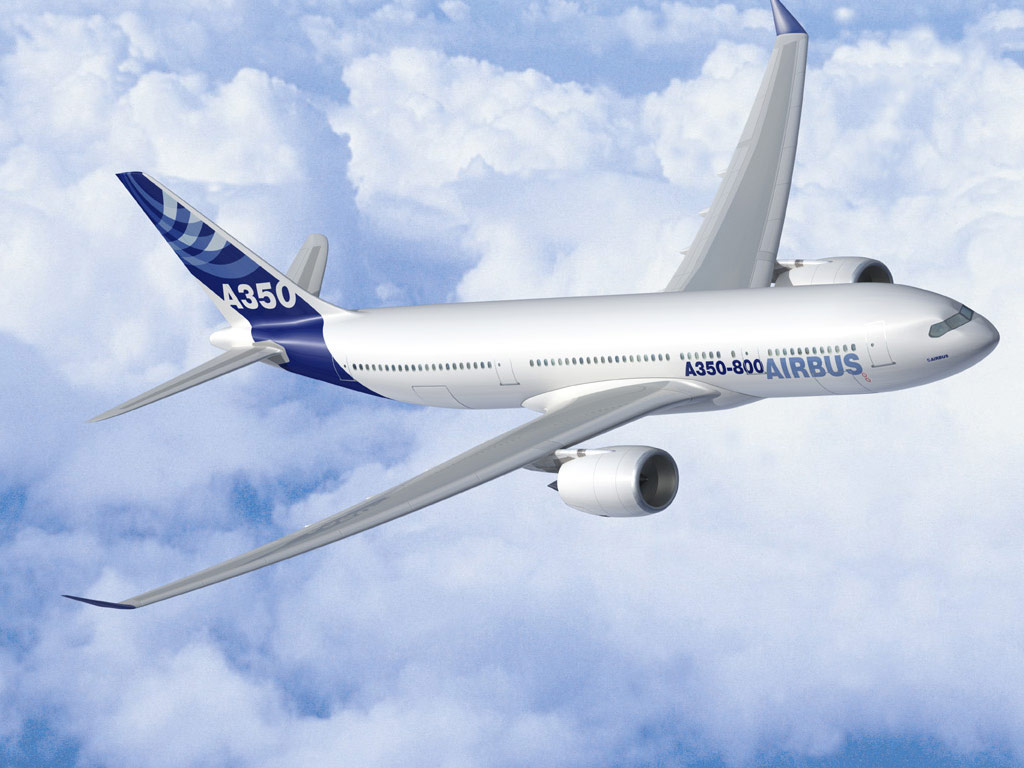
\includegraphics[width=0.25\textwidth]{Figures/Airbus_A350.jpg}
  \caption[Caption for figure in TOC]{Caption for figure.}
  \label{fig:airbus1}
\end{figure}

Make reference to Figure \ref{fig:airbus1}.

\begin{figure}[!htb]
  \begin{subfigmatrix}{2}
    \subfigure[Airbus A320]{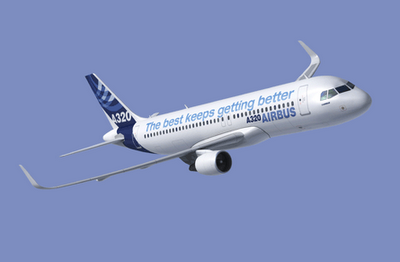
\includegraphics[width=0.49\linewidth]{Figures/Airbus_A320_sharklets.png}}
    \subfigure[Bombardier CRJ200]{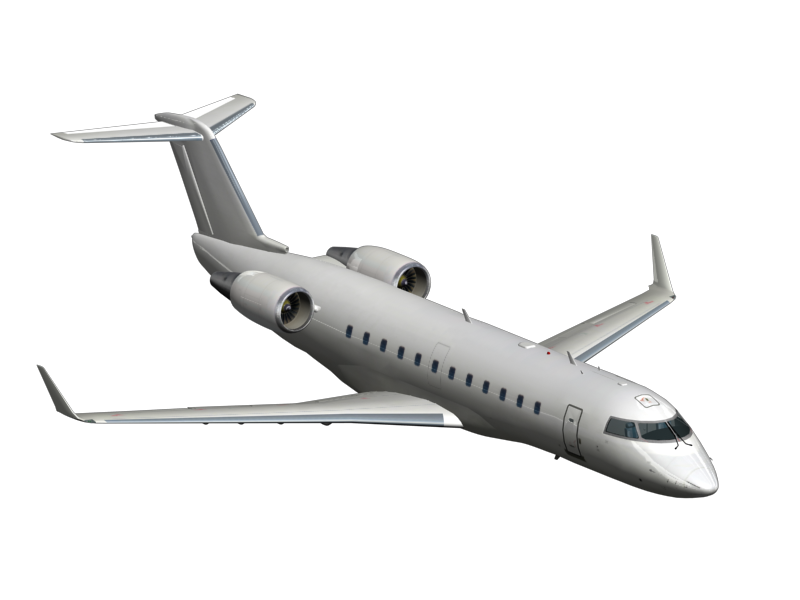
\includegraphics[width=0.49\linewidth]{Figures/Bombardier_CRJ200.png}}
  \end{subfigmatrix}
  \caption{Aircrafts.}
  \label{fig:aircrafts}
\end{figure}

By default, the supported file types are {\it .png,.pdf,.jpg,.mps,.jpeg,.PNG,.PDF,.JPG,.JPEG}.

See \url{http://mactex-wiki.tug.org/wiki/index.php/Graphics_inclusion} for adding support to other extensions.

% ----------------------------------------------------------------------
\section{Equations}
\label{section:equations}

Equations can be inserted in different ways.

The simplest way is in a separate line like this

\begin{equation}
  \frac{{\rm d} q_{ijk}}{{\rm d} t} + {\cal R}_{ijk}({\bf q}) = 0 \,.
\label{eq:ode}
\end{equation}

If the equation is to be embedded in the text. One can do it like this ${\partial {\cal R}}/{\partial {\bf q}}=0$.

It may also be split in different lines like this

\begin{eqnarray}
  {\rm Minimize}   && Y({\bf \alpha},{\bf q}({\bf \alpha}))            \nonumber           \\
  {\rm w.r.t.}     && {\bf \alpha} \,,                                 \label{eq:minimize} \\
  {\rm subject~to} && {\cal R}({\bf \alpha},{\bf q}({\bf \alpha})) = 0 \nonumber           \\
                   &&       C ({\bf \alpha},{\bf q}({\bf \alpha})) = 0 \,. \nonumber
\end{eqnarray}

It is also possible to use subequations. Equations~\ref{eq:continuity}, \ref{eq:momentum} and \ref{eq:energy} form the Naver--Stokes equations~\ref{eq:NavierStokes}.

\begin{subequations}
    \begin{equation}
    \frac{\partial \rho}{\partial t} + \frac{\partial}{\partial x_j}\left( \rho u_j \right) = 0 \,,
    \label{eq:continuity}
    \end{equation}
    \begin{equation}
    \frac{\partial}{\partial t}\left( \rho u_i \right) + \frac{\partial}{\partial x_j} \left( \rho u_i u_j + p \delta_{ij} - \tau_{ji} \right) = 0, \quad i=1,2,3 \,,
    \label{eq:momentum}
    \end{equation}
    \begin{equation}
        \frac{\partial}{\partial t}\left( \rho E \right) + \frac{\partial}{\partial x_j} \left( \rho E u_j + p u_j - u_i \tau_{ij} + q_j \right) = 0 \,.
    \label{eq:energy}
    \end{equation}
\label{eq:NavierStokes}%
\end{subequations}


\cleardoublepage

 % file "Thesis_Results.tex"

%%%%%%%%%%%%%%%%%%%%%%%%%%%%%%%%%%%%%%%%%%%%%%%%%%%%%%%%%%%%%%%%%%%%%%%%
%                                                                      %
%     File: Thesis_Conclusions.tex                                     %
%     Tex Master: Thesis.tex                                           %
%                                                                      %
%     Author: Andre C. Marta                                           %
%     Last modified : 21 Jan 2011                                      %
%                                                                      %
%%%%%%%%%%%%%%%%%%%%%%%%%%%%%%%%%%%%%%%%%%%%%%%%%%%%%%%%%%%%%%%%%%%%%%%%

\chapter{Conclusions}
\label{chapter:conclusions}

Insert your chapter material here...


% ----------------------------------------------------------------------
\section{Achievements}
\label{section:achievements}

The major achievements of the present work...


% ----------------------------------------------------------------------
\section{Future Work}
\label{section:future}

A few ideas for future work...


\cleardoublepage

 % file "Thesis_Conclusions.tex"

% ----------------------------------------------------------------------
%  Appendix (optional)
% ----------------------------------------------------------------------
\appendix
%%%%%%%%%%%%%%%%%%%%%%%%%%%%%%%%%%%%%%%%%%%%%%%%%%%%%%%%%%%%%%%%%%%%%%%%
%                                                                      %
%     File: Thesis_Appendix.tex                                        %
%     Tex Master: Thesis.tex                                           %
%                                                                      %
%     Author: Andre C. Marta                                           %
%     Last modified : 21 Jan 2011                                      %
%                                                                      %
%%%%%%%%%%%%%%%%%%%%%%%%%%%%%%%%%%%%%%%%%%%%%%%%%%%%%%%%%%%%%%%%%%%%%%%%

\chapter{Vector calculus}
\label{chapter:appendixVectors}

In case an appendix if deemed necessary, the document cannot exceed a total of 100 pages...

Some definitions and vector identities are listed in the section below.

% ----------------------------------------------------------------------
\section{Vector identities}
\label{section:vectorIdentities}

\begin{equation}
	\nabla \times \left( \nabla \phi \right) = 0
	\label{eq:cross_nnp}
\end{equation}

\begin{equation}
	\nabla \cdot \left( \nabla \times {\bf u} \right) = 0
	\label{eq:dotCross_nnu}
\end{equation}

\cleardoublepage

 % file "Thesis_Appendix.tex"

% ----------------------------------------------------------------------
%  Bibliography
% ----------------------------------------------------------------------

% Include all references in .bib file, even non-cited ones...
\nocite{*}

% Produces the bibliography section when processed by BibTeX
%
% Bibliography style
% > entries ordered alphabetically
%\bibliographystyle{plain}
% > unsorted with entries appearing in the order in which the citations appear.
%\bibliographystyle{unsrt}
% > entries ordered alphabetically, with first names and names of journals and months abbreviated
%\bibliographystyle{abbrv}
% > entries ordered alphabetically, with reference markers based on authors' initials and publication year
%\bibliographystyle{alpha}
%
% Replacement bibliography styles provided by 'natbib' package
% (plainnat.bst, abbrvnat.bst, unsrtnat.bst )
% > entries ordered alphabetically
\bibliographystyle{plainnat}
% > unsorted with entries appearing in the order in which the citations appear.
%\bibliographystyle{unsrtnat}
% > entries ordered alphabetically, with first names and names of journals and months abbreviated
%\bibliographystyle{abbrvnat}
% > entries ordered alphabetically, with reference markers based on authors' initials and publication year
%\bibliographystyle{alpha}


% External bibliography database file in the BibTeX format
\cleardoublepage
\bibliography{Thesis_bib_DB} % file "Thesis_bib_DB.bib"
% Add entry in the table of contents as chapter
\addcontentsline{toc}{chapter}{\bibname}
\cleardoublepage

% ----------------------------------------------------------------------
\end{document}
% ----------------------------------------------------------------------

